\documentclass[en,black,normal,10pt]{elegantnote}
\usepackage{lipsum} % Required for generating dummy text
\usepackage{tikz}
\usetikzlibrary{bayesnet}
\usetikzlibrary{positioning}
\usepackage{caption}
\usepackage{booktabs}
\usepackage{float}
\usepackage{amsmath}

\usetikzlibrary{trees,matrix,arrows,positioning}

\setlength{\parindent}{0pt}

\title{DSAA 5002 - HW2}

%\version{Fall Semester 2023}

\author{50015976 Ruiming ZHANG}
%\institute{Elegant\LaTeX{} Program}

\date{}

\usetikzlibrary{shapes,arrows}

\begin{document}

\maketitle
% logo
%\centerline{\includegraphics[width=0.2\textwidth]{logo-blue}}

\section*{Q1 [25 Marks]}

Consider the following training data with labels 0 and 1, and three
attributes A, B, and C

\definecolor{Gray}{gray}{0.85} % Define a custom color

\begin{table}[H]
    \centering
    \begin{tabular}{ccccc}
        \hline
        \addlinespace[-0.5ex] % 调整间距 \toprule
        \hline
        id & A & B & C & class \\
        \hline
        1 & 0.62 & yes & yes & 0 \\
        \hline
        2 & 3.84 & no & no & 0 \\
        \hline
        3 & 6.61 & yes & no & 0 \\
        \hline
        4 & 6.87 & yes & no & 0 \\
        \hline
        5 & 7.71 & no & yes & 0 \\
        \hline
        6 & 8.98 & no & yes & 0 \\
        \hline
        7 & 1.77 & yes & no & 0 \\
        \hline
        8 & 2.02 & yes & no & 1 \\
        \hline
        9 & 2.06 & no & yes & 1 \\
        \hline
        10 & 2.66 & no & yes & 1 \\
        \hline
        11 & 3.72 & no & yes & 1 \\
        \hline
        12 & 4.98 & yes & yes & 1 \\
        \hline
        13 & 5.73 & yes & yes & 1 \\
        \hline
        14 & 6.29 & yes & yes & 1 \\
        \hline
        15 & 9.08 & no & no & 1 \\
        \hline
        16 & 9.45 & no & no & 1 \\
        \hline
        \addlinespace[-0.5ex] % 调整间距 \toprule
        \hline
    \end{tabular}
\end{table}

\begin{itemize}
    \item[(a)] (10 marks) Try threshold 2, 5, and 8 for attributes A (that is, use the “A > 2, A < 2”, “A > 5, A < 5”, and “A > 8, A < 8” respectively). Use the Gini score to determine the best one $\theta_a$ among them. Recall:
    \begin{equation*}
        Gini(t) = 1 - \sum_{i = 1}^{c} [p(i|t)]^2  
    \end{equation*}
    \item[(b)] (20 marks) Use $\theta_a$ obtained above, and the Gini score, determine which attributes should firstly be used for developing a decision tree.
\end{itemize}

\subsection*{Solution:}

\paragraph*{(a)} We have: $Info(T) = 1 - (\frac{7}{16})^2 - (\frac{9}{16})^2 = \frac{63}{128} \approx 0.4922$

For threshold 2:

$Info(T_{A<2}) = 1 - \frac{2}{2}^2 - \frac{0}{2}^2 = 0$

$Info(T_{A>2}) = 1 - \frac{5}{14}^2- \frac{9}{14}^2 = \frac{45}{98} \approx 0.4592$

$Info(A_{threshold=2}, T) = \frac{2}{16} \times 0 + \frac{14}{16} \times \frac{45}{98} = \frac{45}{122} \approx 0.4018$

$Gain(A_{threshold=2}, T) = \frac{63}{128} - \frac{45}{122} = \frac{81}{896} \approx 0.0904$

For threshold 5:

$Info(T_{A<5}) = 1 - \frac{3}{8}^2 - \frac{5}{8}^2 = 0$

$Info(T_{A>5}) = 1 - \frac{4}{8}^2- \frac{4}{8}^2 = \frac{45}{98} \approx 0.4592$

$Info(A_{threshold=5}, T) = \frac{8}{16} \times 0 + \frac{8}{16} \times \frac{45}{98} = \frac{45}{122} \approx 0.4018$

$Gain(A_{threshold=5}, T) = \frac{63}{128} - \frac{45}{122} = \frac{81}{896} \approx 0.0904$

For threshold 8:

$Info(T_{A<8}) = 1 - \frac{6}{13}^2 - \frac{7}{13}^2 = 0$

$Info(T_{A>8}) = 1 - \frac{1}{3}^2- \frac{2}{3}^2 = \frac{45}{98} \approx 0.4592$

$Info(A_{threshold=8}, T) = \frac{13}{16} \times 0 + \frac{3}{16} \times \frac{45}{98} = \frac{45}{122} \approx 0.4018$

$Gain(A_{threshold=8}, T) = \frac{63}{128} - \frac{45}{122} = \frac{81}{896} \approx 0.0904$


\section*{Q2 [30 Marks]}

The table below is a small part of the Acute Inflammations Data Set.

\begin{table}[H]
    \begin{tabular}{ll}
        a1 & Temperature of patient (35C-42C) \\
        a2 & Occurrence of nausea (yes, no) \\
        a3 & Lumbar pain (yes, no) \\
        a4 & Urine pushing (continuous need for urination) (yes, no) \\
        a5 & Micturition pains (yes, no) \\
        a6 & Burning of urethra, itch, swelling of urethra outlet (yes, no) \\
        d1 & Decision: Inflammation of urinary bladder (yes, no) \\
        d2 & Decision: Nephritis of renal pelvis origin (yes, no) \\
    \end{tabular}
\end{table}

Here the attributes a1-a6 are observations, and the decisions d1 and d2 are made by a
medical expert. The purpose of studying this data set is to predict presumptive diagnosis
of two disease of the urinary system, namely, “Inflammation of urinary bladder” and
“Nephritis of renal pelvis origin".

\begin{table}[H]
    \centering
    \begin{tabular}{cccccc|cc}
        \hline
        \addlinespace[-0.5ex] % 调整间距 \toprule
        \hline
        a1 & a2 & a3 & a4 & a5 & a6 & d1 & d2 \\
        \hline
        37.3 & no & yes & no & no & no & no & no \\
        \hline
        37.4 & no & no & yes & no & no & yes & no \\
        \hline
        37.5 & yes & yes & no & no & no & no & no \\
        \hline
        37.6 & no & no & yes & yes & yes & yes & yes \\
        \hline
        37.7 & no & no & yes & no & no & yes & no \\
        \hline
        37.7 & no & no & yes & yes & no & yes & no \\
        \hline
        37.7 & no & no & yes & yes & no & yes & no \\
        \hline
        37.8 & no & yes & no & no & no & no & no \\
        \hline
        37.9 & no & no & yes & yes & yes & yes & no \\
        \hline
        37.9 & no & no & yes & no & no & yes & no \\
        \hline
        38.0 & no & yes & yes & no & yes & no & yes \\
        \hline
        38.0 & no & yes & yes & no & yes & no & yes \\
        \hline
        38.1 & no & yes & yes & no & yes & yes & yes \\
        \hline
        38.3 & no & yes & yes & no & yes & no & yes \\
        \hline
        38.5 & no & yes & yes & no & yes & no & no \\
        \hline
        38.7 & no & yes & yes & no & yes & no & yes \\
        \hline
        38.9 & no & yes & yes & no & yes & yes & yes \\
        \hline
        39.0 & no & yes & yes & no & yes & no & yes \\
        \hline
        39.4 & no & yes & yes & no & yes & no & yes \\
        \hline
        39.5 & no & yes & yes & no & yes & no & yes \\
        \hline
        \addlinespace[-0.5ex] % 调整间距 \bottomrule
        \hline
    \end{tabular}
\end{table}

\begin{itemize}
    \item[(a)] (10 marks) Consider the procedures of building a decision tree with Gini score. If we plan only to use the attributes a3 and a5 to predict the decision d2, which attribute should we use first?
    \item[(b)] (20 marks) Use the naïve Bayes algorithm, the attributes a1 (with the threshold $\theta_1$ = 37.95), a2, and a3 only, to predict the decision d2 for the following data of a new patient. (For simplicity you do NOT need to use the Laplacian correction.)
\end{itemize}

\begin{table}[H]
    \centering
    \begin{tabular}{cccccc|cc}
        \hline
        \addlinespace[-0.5ex] % 调整间距 \toprule
        \hline
        a1 & a2 & a3 & a4 & a5 & a6 & d1 & d2 \\
        \hline
        40.0 & yes & no & no & no & no & ? & ? \\
        \hline
        \addlinespace[-0.5ex] % 调整间距 \bottomrule
        \hline
    \end{tabular}
\end{table}

\subsection*{Solution:}

\paragraph*{(a)} Because we only predict the decision d2, we have: $Info(T)=1-\frac{1}{2}^2-\frac{1}{2}^2=0.5$

For attribute a3, we have:

$Info(T_{yes}) = 1 - \frac{9}{13}^2 - \frac{4}{13}^2 = \frac{72}{169} \approx 0.4260$

$Info(T_{no}) = 1 - \frac{1}{7}^2- \frac{6}{7}^2 = \frac{12}{49} \approx 0.2499$

$Info(a3, T) = \frac{13}{20} \times \frac{72}{169} + \frac{7}{20} \times \frac{12}{49} = \frac{33}{91} \approx 0.3626$

$Gain(a3, T) = 0.5 - 0.3626 = 0.1374$

For attribute a5, we have:

$Info(T_{yes}) = 1 - \frac{1}{4}^2 - \frac{3}{4}^2 = \frac{3}{8} = 0.3750$

$Info(T_{no}) = 1 - \frac{9}{16}^2- \frac{7}{16}^2 = \frac{63}{128} \approx 0.4922$

$Info(a5, T) = \frac{4}{20} \times \frac{3}{8} + \frac{16}{20} \times \frac{63}{128} = \frac{15}{32} \approx 0.4688$

$Gain(a5, T) = 0.5 - 0.4688 = 0.0312$

We can see $Gain(a3, T) > Gain(a5, T)$, so we should use a3 first.

\paragraph*{(b)} Because we have:

For attribute a1:

$P(a1>\theta_1|d2=yes)=\frac{9}{10}=0.9$

$P(a1<\theta_1|d2=yes)=\frac{1}{10}=0.1$

$P(a1>\theta_1|d2=no)=\frac{1}{10}=0.1$

$P(a1<\theta_1|d2=no)=\frac{9}{10}=0.9$

For attribute a2:

$P(a2=yes|d2=yes)=\frac{0}{10}=0$

$P(a2=no|d2=yes)=\frac{10}{10}=1$

$P(a2=yes|d2=no)=\frac{1}{10}=0.1$

$P(a2=no|d2=no)=\frac{9}{10}=0.9$

For attribute a3:

$P(a3=yes|d2=yes)=\frac{9}{10}=0.9$

$P(a3=no|d2=yes)=\frac{1}{10}=0.1$

$P(a3=yes|d2=no)=\frac{4}{10}=0.4$

$P(a3=no|d2=no)=\frac{6}{10}=0.6$

Then we have:

{
    \setlength{\abovedisplayskip}{-10pt}
    \setlength{\belowdisplayskip}{0pt}

    \begin{flalign*}
        P &= P(a1>\theta_1,a2=yes,a3=no) && \\
            &= P(a1>\theta_1) \times P(a2=yes)\times P(a3=no) \\
            &=0.00875
    \end{flalign*}

    \begin{flalign*}
        P_1 &= P(a1>\theta_1,a2=yes,a3=no|d2=yes) && \\
            &= P(a1>\theta_1|d2=yes) \times P(a2=yes|d2=yes)\times P(a3=no|d2=yes) \\
            &=0.9 \times 0 \times 0.1 \\
            &=0
    \end{flalign*}

    \begin{flalign*}
        P_2 &= P(a1>\theta_1,a2=yes,a3=no|d2=no) && \\
            &= P(a1>\theta_1|d2=no) \times P(a2=yes|d2=no)\times P(a3=no|d2=no) \\
            &=0.1 \times 0.1 \times 0.6 \\
            &=0.006
    \end{flalign*}
}

Thus: 

{
    \setlength{\abovedisplayskip}{-10pt}
    \setlength{\belowdisplayskip}{0pt}

    \begin{flalign*}
        &P(d2=yes|a1>\theta_1,a2=yes,a3=no) \\
            &=\frac{P_1 \times P(d2=yes)}{P} && \\
            &=\frac{0 \times 0.5}{0.00875} \\
            &=0
    \end{flalign*}

    \begin{flalign*}
        &P(d2=no|a1>\theta_1,a2=yes,a3=no) \\
            &=\frac{P_2 \times P(d2=no)}{P} && \\
            &=\frac{0.006 \times 0.5}{0.00875} \\
            &=0.3429
    \end{flalign*}
}

Hence, the decision of d2 is no.
\section*{Q3 [15 Marks]}

There is a BBN below, which comprises four Random Variables(RV).
Each RV is a Boolean RV

\begin{center}
    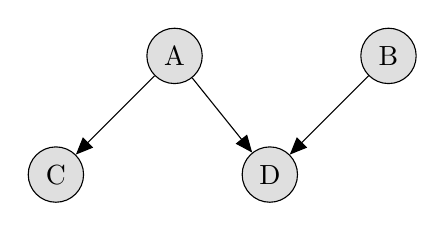
\begin{tikzpicture}
        % Define nodes
        \node[obs] (A) {A};
        \node[obs, right=2cm of A] (B) {B};
        \node[obs, below left=1cm and 1cm of A] (C) {C};
        \node[obs, right=2cm of C] (D) {D};
        % Connect nodes
        \edge {A} {C};
        \edge {A,B} {D};
    \end{tikzpicture}
\end{center}

\begin{table}[H]
    \centering
    \begin{tabular}{lll}
        \(P(A) = 0.1\) & \(P(B) = 0.5\) & \(P(C|A) = 0.7\) \\
        \(P(C|\lnot A) = 0.2\) & \(P(D|A, B) = 0.9\) & \(P(D|\lnot A, B) = 0.6\) \\
        \(P(D|A, \lnot B) = 0.7\) & \(P(D|\lnot A, \lnot B) = 0.3\)
    \end{tabular}
\end{table}

\begin{itemize}
    \item[(a)] (7 marks) What is $P(\lnot A, B, \lnot C, D)$?
    \item[(b)] (8 marks) What is $P(A | B, C, D)$?
\end{itemize}

\subsection*{Solution:}

\paragraph*{(a)} According to the BBN above, we have:

{
    \setlength{\abovedisplayskip}{-10pt}
    \setlength{\belowdisplayskip}{0pt}

    \begin{flalign*}
        P(\lnot A, B, \lnot C, D) &= P(B, D|\lnot A, \lnot C) \times P(\lnot A, \lnot C)&& \\
            &= P(B, D | \lnot A) \times P(\lnot C | \lnot A) \times P(\lnot A) && \\
            &= P(D|\lnot A B) \times P(B) \times [1 - P(C | \lnot A)] \times [1 - P(A)] && \\
            &= 0.6 \times 0.5 \times (1-0.2) \times (1-0.1) && \\
            &= 0.216
    \end{flalign*}
}

\paragraph*{(b)} According to the BBN above, we have:

{
    \setlength{\abovedisplayskip}{-10pt}
    \setlength{\belowdisplayskip}{0pt}

    \begin{flalign*}
        P(A | B, C, D) &= \frac{P(A, B, C, D)}{P(B, C, D)} && \\
            &= \frac{P(B, D | A, C) \times P(A, C)}{P(B, C, D)} && \\
            &= \frac{P(B, D | A) \times P(A, C)}{P(B, D) \times P(C)} && \\
            &= \frac{P(D | A, B) \times P(B) \times [P(C | A) \times P(A)]}{[P(B, D, A) + P(B, D, \lnot A)] \times P(C)} && \\
            &= \frac{P(D | A, B) \times P(B) \times [P(C | A) \times P(A)]}{[P(D | A, B) \times P(A, B) + P(D | \lnot A, B) \times P(\lnot A, B)] \times P(C)} && \\
        \end{flalign*}
}

Except for \( P(C) \), all other variables are known. According to Total Probability Formula, we have:

{
    \setlength{\abovedisplayskip}{-10pt}
    \setlength{\belowdisplayskip}{0pt}

    \begin{flalign*}
        P(C) &= P(C, A) + P(C, \lnot A) && \\
            &= P(C | A) \times P(A) + P(C | \lnot A) \times P(\lnot A) && \\
            &= 0.7 \times 0.1 + 0.2 \times 0.9 && \\
            &= 0.25
    \end{flalign*}
}

Hence:

$P(A | B, C, D) = \frac{0.9 \times 0.5 \times [0.7 \times 0.1]}{[0.9 \times 0.1 \times 0.5 + 0.6 \times 0.9 \times 0.5] \times 0.25} = 0.4$
\section*{Q4 [30 Marks]}

Consider a simple neural network with a single hidden layer. 
The input layer consists of three-dimensional \( \mathbf{x} = (x_1, x_2, x_3)^T \). 
The hidden layer includes two-dimensional \( \mathbf{h} = (h_1, h_2) \). 
The output layer includes one scalar \( o \). 
We ignore bias terms for simplicity.

We use linear rectified (ReLU) as activation function \textbf{for the hidden and output layer BOTH}.
\begin{equation*}
    \text{ReLU}(x) = \max(0, x)
\end{equation*}
\begin{equation*}
    \text{ReLU}'(x) = 
        \begin{cases} 
        1, & \text{if } x > 0 \\
        0, & \text{if } x \leq 0 
        \end{cases}
\end{equation*}

Moreover, denote the loss function (also called error in slides) by \( \mathbf{J}(o, t) = \frac{1}{2} |o - t|^2 \).
where \( t \) is the associated label (target) value for scalar output \( o \).
Denote by \( W \) and \( V \) weight matrices connecting input and hidden layer, and hidden layer and output respectively.
They are \textbf{initialized} (i.e., the initial condition before the first updating round) as follows:
\begin{equation}
W = \begin{bmatrix}
1 & 0 & 1 \\
-3 & -1 & 0 \\
\end{bmatrix}, 
V = \begin{bmatrix}
0 & 1
\end{bmatrix},
\end{equation}

Now, try to solve the following parts.

\begin{itemize}
    \item[(a)] (5 marks) Write out symbolically (thus, no need to plug in the specific values of \( W \) and \( V \) just yet) the mapping \( \mathbf{x} \rightarrow o \) using ReLU, \( W \), \( V \).
    \item[(b)] (10 marks) Given the condition \( \mathbf{x} = (1, 2, 1)^T, t = 1 \), compute the numerical output value \( o \), clearly show all intermediate steps. You can reuse the results of the previous question.
    \item[(c)] (15 marks) Compute the gradient of the loss function with respect to the \( V \) weights, and evaluate the gradients at specific \( \mathbf{x} = (1, 2, 1)^T, t = 1 \).
\end{itemize}

Forward Pass

1. Hidden Layer Calculation: 

    The output of the hidden layer can be computed as \( \mathbf{h} = \text{ReLU}(W \cdot \mathbf{x}) \).
    
    Given \( W = \begin{pmatrix} 1 & 0 & 1 \\ -3 & -1 & 0 \end{pmatrix} \) and \( \mathbf{x} = \begin{pmatrix} 1 \\ 2 \\ 1 \end{pmatrix} \),
    
    \[
    \mathbf{h} = \text{ReLU}\left(\begin{pmatrix} 1 & 0 & 1 \\ -3 & -1 & 0 \end{pmatrix} \begin{pmatrix} 1 \\ 2 \\ 1 \end{pmatrix}\right)
    = \text{ReLU}\left(\begin{pmatrix} 2 \\ -5 \end{pmatrix}\right)
    = \begin{pmatrix} 2 \\ 0 \end{pmatrix}
    \]

2. Output Layer Calculation: 

    The output \( o \) can be computed as \( o = \text{ReLU}(V \cdot \mathbf{h}) \).
    
    Given \( V = \begin{pmatrix} 0 & 1 \end{pmatrix} \) and \( \mathbf{h} = \begin{pmatrix} 2 \\ 0 \end{pmatrix} \),
    
    \[
    o = \text{ReLU}\left(\begin{pmatrix} 0 & 1 \end{pmatrix} \begin{pmatrix} 2 \\ 0 \end{pmatrix}\right)
    = \text{ReLU}(0)
    = 0
    \]

So, the numerical output value \( o \) would be 0 given the condition \( \mathbf{x} = (1, 2, 1)^T \) and \( t = 1 \).

To compute the gradient of the loss function with respect to the \( V \) weights, we first need to define the loss function and then use backpropagation to find the gradients.

Loss Function:
The given loss function is 
\[
J(o, t) = \frac{1}{2} |o - t|^2
\]
where \( o \) is the predicted output and \( t \) is the target value.

Backpropagation for Computing Gradient:
We want to find \( \frac{\partial J}{\partial V} \).

1. First, compute \( \frac{\partial J}{\partial o} \) (the derivative of the loss function with respect to the output):
\[
\frac{\partial J}{\partial o} = o - t
\]

2. Next, compute \( \frac{\partial o}{\partial V} \) (the derivative of the output with respect to the \( V \) weights). Since \( o = \text{ReLU}(V \cdot h) \), and \( h = (2, 0)^T \) (from our earlier calculation), \( \frac{\partial o}{\partial V} = h \) if \( o > 0 \) and \( \frac{\partial o}{\partial V} = 0 \) otherwise.

3. Finally, use the chain rule to find \( \frac{\partial J}{\partial V} \):
\[
\frac{\partial J}{\partial V} = \frac{\partial J}{\partial o} \times \frac{\partial o}{\partial V}
\]

Evaluate the Gradients:
1. \( \frac{\partial J}{\partial o} = o - t = 0 - 1 = -1 \)
2. \( \frac{\partial o}{\partial V} = (2, 0)^T \) (because \( o = 0 \) which is not greater than 0)
3. \( \frac{\partial J}{\partial V} = -1 \times (2, 0)^T = (-2, 0) \)

So, the gradient of the loss function with respect to the \( V \) weights is \( (-2, 0) \).


\end{document}
